

En este capítulo se presenta la planificación del proyecto, abordando el alcance definido, los periodos de realización de tareas y los diversos ámbitos de gestión: temporal, de riesgos, de comunicaciones e información, y de partes interesadas. El objetivo de esta planificación es establecer una hoja de ruta estructurada que permita el cumplimiento de todos los objetivos del proyecto dentro de los plazos establecidos.

\section{Alcance}

Este proyecto aborda el desarrollo de un sistema basado en agentes LLM implementado sobre una solución software propia de LKS Next, el cual deberá responder a consultas formuladas en lenguaje natural que un desarrollador recién incorporado podría plantear durante su proceso de integración al proyecto. Con ello se pretende investigar el comportamiento de diversas arquitecturas de agentes definidas en el Capítulo \ref{ch:chap2} y evaluar su viabilidad para su futura incorporación en los procesos productivos de la empresa.

En dicho sistema, se implementarán diversas modalidades de interacción entre agentes especializados en fuentes de datos específicas, evaluando la eficacia de los distintos patrones de comunicación entre dichos componentes.

Cabe destacar que el alcance del proyecto no está definido en su totalidad, dada la complejidad de estimación inherente a su naturaleza exploratoria y al uso de tecnologías emergentes. Para mitigar riesgos en el desarrollo, se ha establecido un protocolo preventivo que contempla reuniones quincenales de seguimiento y control.

\subsection{Objetivos concretos del proyecto}
\label{chap3:objetivos}

Para facilitar el logro del objetivo principal, se han identificado y definido los siguientes objetivos específicos que estructuran el avance progresivo del proyecto:

\begin{itemize}
  \item\textbf{Estudio de arquitecturas agénticas: }realizar un análisis de las diversas arquitecturas de agentes, considerando distintas estrategias de interacción y mecanismos de acceso a fuentes de información.
\item\textbf{Desarrollo de sistema de onboarding: }implementar un prototipo que simule una aplicación integrada en la empresa como parte de una iniciativa organizacional más amplia en este ámbito, aplicando las arquitecturas propuestas sobre un proyecto software corporativo. El objetivo consiste en analizar su eficacia en la asistencia a nuevos integrantes durante su proceso de incorporación a la empresa.
  \item\textbf{Integración del Model Context Protocol: }exploración de las características y beneficios que aporta la implementación del protocolo MCP, con el objetivo de realizar una valoración objetiva para su posible integración en el entorno profesional de la empresa.
  \item\textbf{Evaluación de agentes: }desarrollar un sistema de evaluación para proporcionar métricas comparativas cuantificables sobre el rendimiento de los diferentes enfoques de agentes. 
  \item\textbf{Valoración de ajuste de agentes: }analizar la relación coste-beneficio asociada al proceso de ajuste fino de modelos LLM para su aplicación en agentes concretos.
\end{itemize}

Adicionalmente, el proyecto contempla desarrollar el sistema de onboarding incorporando en la medida de lo posible en su base de conocimiento la metodología de trabajo implementada en la empresa. Mediante la adhesión a los estándares definidos en un entorno profesional real, se pretende garantizar que los resultados obtenidos constituyan un reflejo de la viabilidad de implementación y eficacia de proyectos similares en un sistema de explotación. 

\subsection{Fases del proyecto}
Tal y como se ha mencionado anteriormente, el alcance del proyecto no está completamente definido debido a su naturaleza exploratoria. Consecuentemente, se propone un ciclo de vida iterativo-incremental con iteraciones de aproximadamente dos semanas de duración, permitiendo una adaptación progresiva a los requisitos emergentes.

La primera iteración se centra en la captura de requisitos del proyecto, donde se explorará y definirá el alcance del sistema de agentes a desarrollar. Complementariamente, se realizará un estudio de las arquitecturas de agentes más relevantes para determinar los enfoques técnicos óptimos para la implementación. Tras establecer estas bases, la segunda iteración abordará la implementación de un sistema de agentes mínimo que contenga la estructura general del sistema, proporcionando un marco operativo inicial.

Con este sistema mínimo implementado, la tercera iteración corresponderá al desarrollo de un mecanismo de evaluación, con el objetivo de establecer métricas que permitan mejorar el sistema en la cuarta iteración, donde se aplicarán las optimizaciones identificadas. 

Finalmente, la quinta iteración se dedicará a la implementación de mejoras sobre el sistema base. Se contemplan tanto arquitecturas de agentes adicionales como el ajuste fino de un modelo LLM para su integración en el flujo agéntico. 

Gracias a la implementación del ciclo de vida iterativo, se logra la consecución de los objetivos del proyecto de forma progresiva y estructurada. Este enfoque permite obtener retroalimentación constante por parte de los directores del proyecto durante cada iteración, facilitando así la posibilidad de reorientar la dirección del trabajo ante la aparición de posibles contratiempos.

\subsection{Descomposición de tareas}
La Estructura de Descomposición de Trabajo (EDT) se ha diseñado considerando el ciclo de vida iterativo-incremental adoptado. La Figura \ref{fig:edt} ilustra un diagrama de los paquetes de trabajo, seguido de la explicación detallada de las tareas individuales de cada paquete.

\begin{figure}[hbtp]
  \centering
  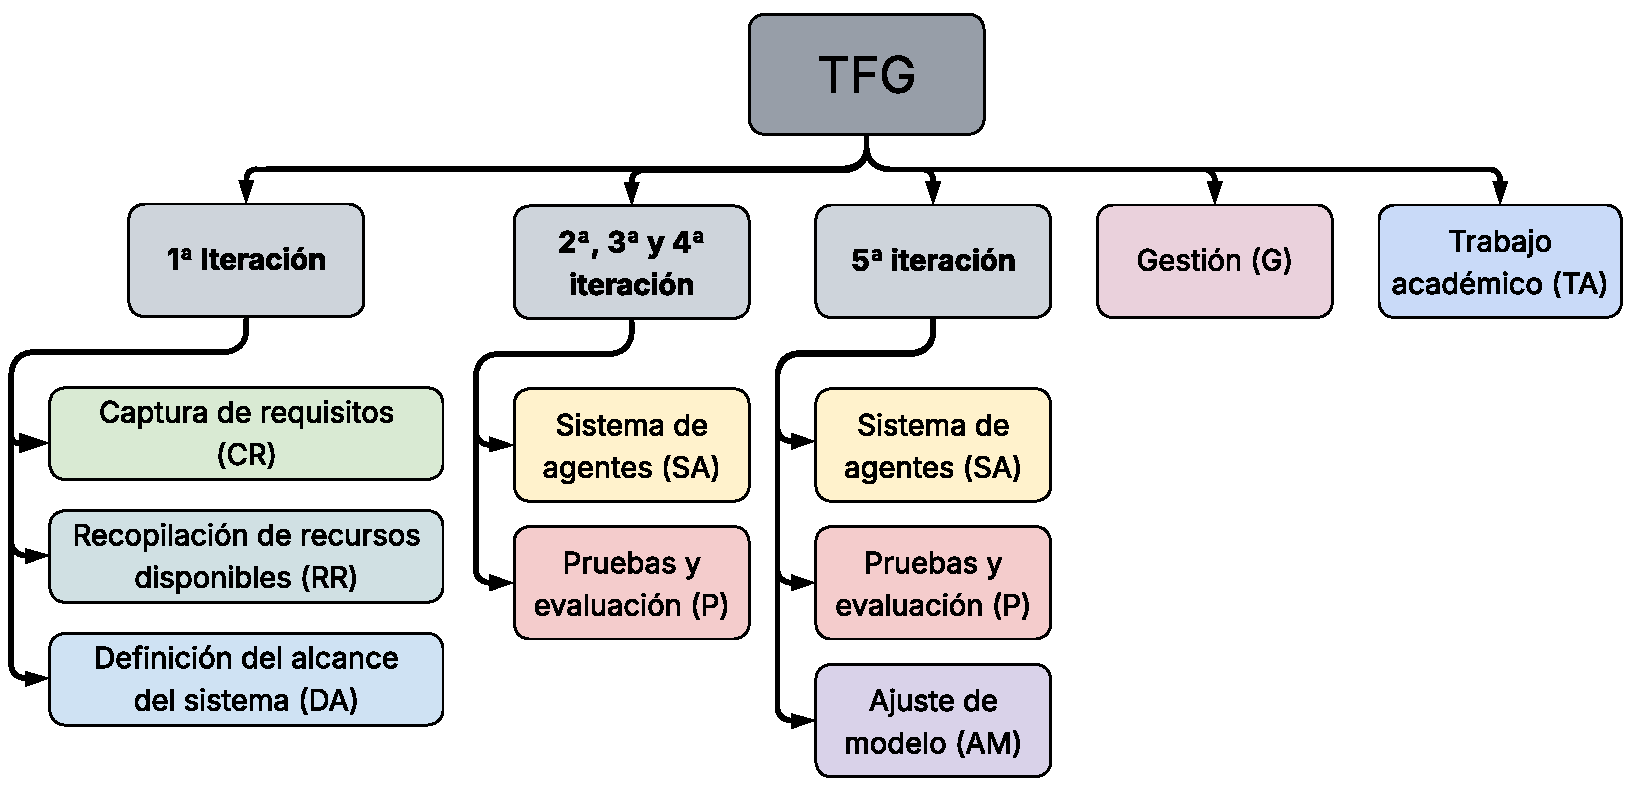
\includegraphics[scale=0.6]{figures/edt_mod.pdf}
  \caption{Estructura de Descomposición de Trabajo (EDT) del proyecto}
  \label{fig:edt}
\end{figure}

\begin{itemize}
  \item\textbf{1ª iteración - Definición de alcance, requisitos y bases del proyecto: }establecimiento de los fundamentos del proyecto.
    \begin{itemize}
      \item\textbf{Captura de requisitos (CR):} actividades orientadas a la definición de los requisitos necesarios para el desarrollo del proyecto.
            \begin{itemize}
          \item\textbf{Definición de requisitos del sistema:} identificación y documentación de los requisitos funcionales y no funcionales que debe cumplir el proyecto, validados con los directores al inicio del mismo.
          \item\textbf{Elicitación de requisitos del dominio:} recopilación de las tipologías de consultas que el sistema debe resolver mediante un cuestionario electrónico dirigido al personal técnico para definir el alcance funcional del sistema.
        \end{itemize}
      \item\textbf{Recopilación de recursos disponibles (RR):} actividades centradas en la selección y generación de recursos esenciales para el desarrollo.
        \begin{itemize}
          \item\textbf{Selección de proyecto software:} identificación y documentación del proyecto software sobre el que se desarrollará el sistema.
          \item\textbf{Generación de recursos:} elaboración de documentación complementaria para la implementación del sistema de agentes.
        \end{itemize}
      \item\textbf{Definición del alcance del sistema de agentes (DA):} delimitación del alcance considerando implementaciones previas y trabajo académico existente.
    \begin{itemize}
          \item\textbf{Investigación de arquitecturas del estado del arte:} análisis de las arquitecturas relevantes documentadas en la literatura académica.
          \item\textbf{Exploración de proyectos similares:} estudio de implementaciones similares en proyectos software y procesos de onboarding.
    \end{itemize}
      \end{itemize}
  \item\textbf{2ª iteración - Implementación del sistema base: }desarrollo del núcleo funcional del sistema con las capacidades mínimas necesarias.
    \begin{itemize}
      \item\textbf{Sistema de agentes (SA):} actividades centradas en el diseño e implementación de un sistema de agentes LLM para asistencia en proyectos software.
        \begin{itemize}
          \item\textbf{Diseño del sistema:} conceptualización e implementación básica de los módulos fundamentales del sistema.
          \item\textbf{Implementación de agentes especializados:} desarrollo de agentes adaptados a las diversas fuentes de información disponibles.
          \item\textbf{Sistema de comunicación mínima:} creación de un mecanismo básico de orquestación para los agentes implementados.
        \end{itemize}
      \item\textbf{Pruebas y evaluación (P):} actividades destinadas a verificar y analizar el rendimiento de los módulos implementados.
        \begin{itemize}
        \item\textbf{Pruebas automatizadas:} desarrollo de pruebas unitarias para algoritmos críticos de los agentes especializados.
        \item\textbf{Integración continua:} implementación de un flujo de trabajo automatizado para la ejecución de pruebas unitarias.
      \end{itemize}
    \end{itemize}
  \item\textbf{3ª iteración - Desarrollo de capacidades de evaluación: }establecimiento de mecanismos de medición y evaluación para cuantificar el rendimiento y guiar las mejoras posteriores del sistema.
    \begin{itemize}
      \item\textbf{Sistema de agentes (SA):} actividades centradas en el diseño e implementación de un sistema de agentes LLM para asistencia en proyectos software.
        \begin{itemize}
          \item\textbf{Sistema de evaluación:} implementación de mecanismos de evaluación automática sobre el sistema mínimo.
          \item\textbf{Captura de datos de evaluación:} anotación manual de ejemplos representativos para evaluar el rendimiento del sistema. 
        \end{itemize}
      \item\textbf{Pruebas y evaluación (P):} actividades destinadas a verificar y analizar el rendimiento de los módulos implementados.
        \begin{itemize}
          \item\textbf{Evaluación del sistema mínimo: } ejecución de evaluaciones automatizadas e identificación de elementos clave para mejoras posteriores.
        \end{itemize}
    \end{itemize}
  \item\textbf{4ª iteración - Optimización y refinamiento: }mejora del sistema existente mediante la aplicación de optimizaciones identificadas a través de la evaluación previa.
    \begin{itemize}
      \item\textbf{Sistema de agentes (SA):} actividades centradas en el diseño, implementación y evaluación de un sistema de agentes LLM para asistencia en proyectos software.
        \begin{itemize}
          \item\textbf{Mejora de agentes:} refinamiento de los agentes implementados para optimizar su rendimiento según las métricas establecidas.
          \item\textbf{Variaciones de orquestación:} análisis e implementación de estrategias alternativas de orquestación. 
        \end{itemize}
      \item\textbf{Pruebas y evaluación (P):} actividades destinadas a verificar y analizar el rendimiento de los módulos implementados.
        \begin{itemize}
          \item\textbf{Evaluación comparativa:} ejecución de evaluaciones automatizadas y análisis comparativo respecto a la iteración anterior.
        \end{itemize}
    \end{itemize}
\item\textbf{5ª iteración - Exploración de mejoras: }implementación de técnicas especializadas y arquitecturas alternativas para maximizar las capacidades del sistema.
    \begin{itemize}
      \item\textbf{Sistema de agentes (SA):} actividades centradas en el diseño e implementación de un sistema de agentes LLM para asistencia en proyectos software.
        \begin{itemize}
          \item\textbf{Arquitecturas de interacción alternativas:} implementación y evaluación de mecanismos adicionales de interacción entre agentes.
          \item\textbf{Módulos de memoria:} integración de sistemas de memoria y evaluación de su impacto en el rendimiento global. 
          \item\textbf{Agentes avanzados:} desarrollo de un agente con un proceso de ejecución extenso para el análisis del coste-beneficio.
          \item\textbf{Incorporación del modelo ajustado:} desarrollo de adaptadores e integración del modelo en el sistema existente.
        \end{itemize}
      \item\textbf{Ajuste de modelo (AM):} actividades orientadas al entrenamiento especializado de un modelo para un agente específico.
      \begin{itemize}
        \item\textbf{Selección del agente:} identificación justificada del agente candidato para el ajuste del modelo.
        \item\textbf{Extracción de datos:} recopilación automatizada de datos de entrenamiento.
        \item\textbf{Entrenamiento del modelo:} diseño y ejecución del ciclo de entrenamiento del modelo LLM seleccionado.
      \end{itemize}
      \item\textbf{Pruebas y evaluación (P):} actividades destinadas a verificar y analizar el rendimiento de los módulos implementados.
        \begin{itemize}
          \item\textbf{Evaluación comparativa: } análisis del rendimiento de las nuevas características respecto al sistema precedente.
        \end{itemize}
    \end{itemize}
  \item\textbf{Gestión (G):} 
    \begin{itemize}
      \item\textbf{Planificación (PL):} establecimiento de directrices, objetivos y actividades para el desarrollo óptimo del proyecto.
      \item\textbf{Seguimiento y control (SC):} monitorización periódica mediante reuniones bisemanales con los directores del proyecto.
    \end{itemize}
  \item\textbf{Trabajo académico (TA):}
    \begin{itemize}
      \item\textbf{Memoria (M):} elaboración del documento académico que recoge todo el trabajo realizado.
      \item\textbf{Defensa (D):} preparación de la presentación y defensa del proyecto ante el tribunal evaluador.
    \end{itemize}
\end{itemize}

\section{Periodos de realización de tareas e hitos}
En este apartado se detallan las dependencias entre las diferentes tareas, así como la estimación de duración y fechas de cada una de ellas.

\subsection{Dependencias entre tareas}
Las dependencias de los paquetes de trabajo del proyecto requieren una ejecución secuencial planificada. La Figura \ref{fig:dependencias} ilustra dichas dependencias.


\begin{figure}[hbtp]
  \centering
  \hspace{-3cm}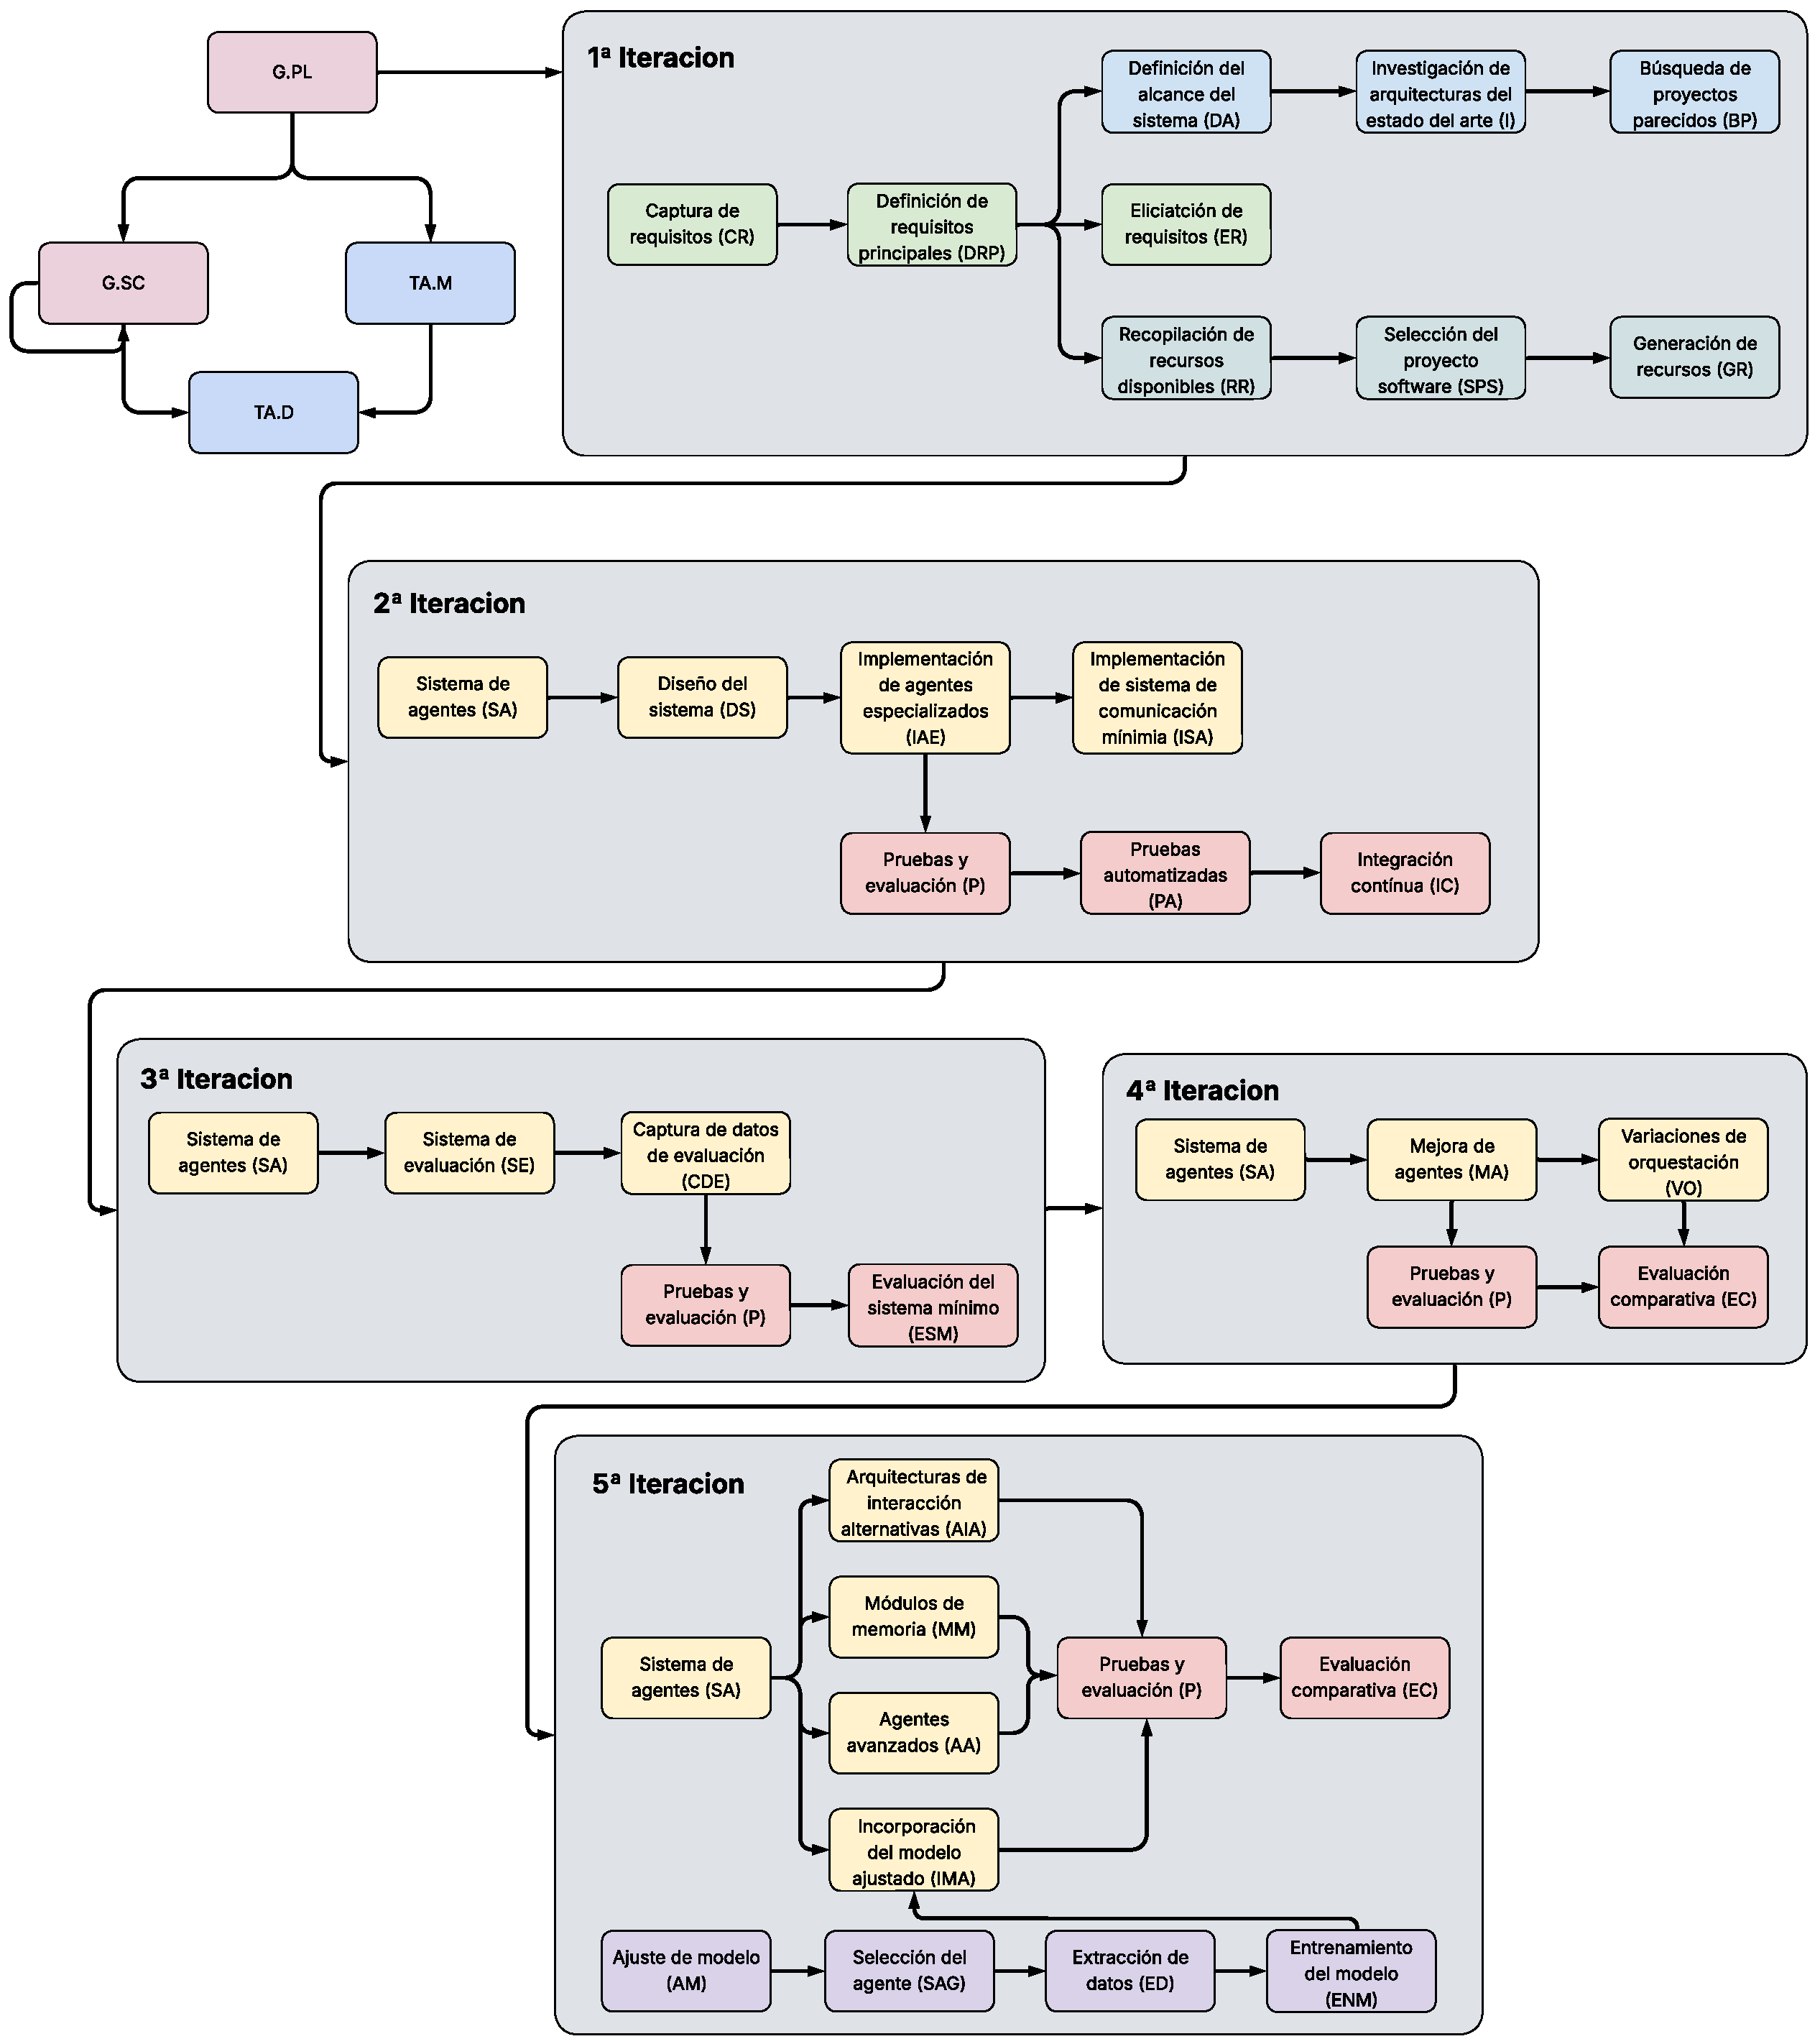
\includegraphics[scale=0.4325]{figures/dep_mod.pdf}%
  \caption{Dependencias entre tareas del proyecto}
  \label{fig:dependencias}
\end{figure}

El proyecto se inicia con la elaboración de la planificación general, estableciendo el alcance del proyecto, fechas y recursos horarios disponibles. La primera iteración aborda la captura de requisitos del proyecto (CR), que define los requisitos del sistema (DRP) y procede posteriormente con los paquetes DA, ER y RR.

La segunda iteración desarrolla el sistema base de agentes (SA), comenzando por el diseño (DS) para continuar con la implementación (IAE, ISA). Una vez implementado, se ejecutan las pruebas automatizadas (PA) y su integración continua (IC).

Las iteraciones tercera y cuarta mantienen una estructura similar, comenzando con la implementación (SA) seguida de pruebas (P). La tercera iteración se centra en el sistema de evaluación, desarrollando primero el mecanismo (SE) para posteriormente anotar los datos de evaluación correspondientes (CDE). La cuarta iteración realiza inicialmente la mejora de agentes (MA) y posteriormente las variaciones de orquestación (VO), manteniendo este orden secuencial para evitar que las mejoras de agentes individuales introduzcan sesgos en los resultados de las variaciones de orquestación. Es importante completar la tercera iteración antes de iniciar la cuarta, ya que modificar los datos de evaluación comprometería la objetividad del análisis.

La quinta iteración comprende cuatro tareas independientes (AIA, MM, AA, AM) que se evalúan individualmente (P) antes de realizar la comparación con las demás versiones del sistema (EC).

Paralelamente, tras finalizar la planificación inicial se inician el seguimiento y control (SC) y la redacción de la memoria (M). Una vez completada la memoria y validado el proyecto durante el proceso de seguimiento y control, se procede con la preparación de la defensa (D).

\subsection{Diagrama de Gantt}

La Figura \ref{fig:gantt} muestra el diagrama de Gantt, donde se visualiza de manera aproximada la distribución temporal a cada paquete de trabajo durante el transcurso del proyecto. Los rombos negros señalan los hitos clave que se detallan en la Sección \ref{sec:hitos}.

\definecolor{crcolor}{HTML}{6aa84f}
\definecolor{rrcolor}{HTML}{45818e}
\definecolor{dacolor}{HTML}{3d85c6}
\definecolor{sacolor}{HTML}{f1c232}
\definecolor{pcolor}{HTML}{cc0000}
\definecolor{amcolor}{HTML}{674ea7}
\definecolor{mdcolor}{HTML}{6d9eeb}

\begin{figure}[hbtp]
  \noindent\hspace*{-2.5cm}
  \begin{ganttchart}[
    vgrid,
    hgrid,
    title label font=\bfseries,
    title height=1,
    bar height=0.6,
    x unit=0.15cm, 
    y unit title=0.7cm,
    y unit chart=0.6cm,
    time slot format=isodate,
    bar label node/.style={rotate=30, anchor=east},  % Inclina las etiquetas 45 grados
    milestone/.style={
        shape=diamond,
        inner sep=2pt,
        draw=black,
        fill=black
    }
  ]{2025-02-25}{2025-06-30}
  
  \gantttitle{Proyecto 2025}{126} \\
  \gantttitle{Feb}{4}\gantttitle{Mar}{31}\gantttitle{Abr}{30}\gantttitle{May}{31}\gantttitle{Jun}{30} \\
  
  % Fila de hitos con rombos negros
  \ganttmilestone{}{2025-02-25} 
  \ganttmilestone{}{2025-03-20} 
  \ganttmilestone{}{2025-04-01} 
  \ganttmilestone{}{2025-04-15} 
  \ganttmilestone{}{2025-04-29} 
  \ganttmilestone{}{2025-05-27} 
  \ganttmilestone{}{2025-06-14} \\
  
  % Barras regulares
  \ganttbar[bar/.style={fill=crcolor!70}]{Planif.}{2025-02-25}{2025-02-28} \\
  \ganttbar[bar/.style={fill=crcolor!70}]{Seg. y cont.}{2025-02-28}{2025-06-14} \\
  \ganttbar[bar/.style={fill=crcolor!70}]{C. requisitos}{2025-02-28}{2025-03-20} \\
  \ganttbar[bar/.style={fill=rrcolor!70}]{R. recursos}{2025-02-28}{2025-03-20} \\
  \ganttbar[bar/.style={fill=dacolor!70}]{D. alcance}{2025-02-28}{2025-03-20} \\
  \ganttbar[bar/.style={fill=sacolor!70}]{S. agentes}{2025-03-20}{2025-05-27} \\
  \ganttbar[bar/.style={fill=pcolor!70}]{Pruebas}{2025-03-20}{2025-05-27} \\
  \ganttbar[bar/.style={fill=amcolor!70}]{A. modelo}{2025-05-13}{2025-05-27} \\
  \ganttbar[bar/.style={fill=mdcolor!70}]{Memoria}{2025-03-20}{2025-06-14} \\
  \ganttbar[bar/.style={fill=mdcolor!70}]{Defensa}{2025-06-14}{2025-06-30} \\
  
  \end{ganttchart}
  \caption{Diagrama de Gantt del proyecto}
  \label{fig:gantt}
\end{figure}
El proyecto se inicia con el paquete de planificación, seguido de la activación del seguimiento y control del proyecto junto con la primera iteración.

A partir de la segunda iteración se desarrollan los paquetes del sistema de agentes y evaluación, que se extienden hasta la quinta iteración. Paralelamente se inicia la redacción de la memoria, al disponerse de material suficiente para los primeros capítulos.

El paquete de ajuste de modelo está planificado para la segunda mitad de la quinta iteración, correspondiente a las últimas dos semanas de implementación. Finalmente, se dedican dos semanas exclusivamente a la memoria, seguidas de la preparación de la defensa.

Esta distribución temporal permite enfocar los esfuerzos según las prioridades de cada fase: planificación y definición del alcance inicialmente, implementación del sistema en la fase intermedia, y trabajo académico al final, manteniendo una redacción continua de la memoria a lo largo del desarrollo.

\subsection{Hitos}\label{sec:hitos}

En la Tabla \ref{tab:hitos} se detallan los hitos establecidos para el desarrollo del proyecto. Estos hitos intermedios permiten evaluar el progreso alcanzado y ajustar el alcance en caso necesario, aspecto fundamental dada la incertidumbre inherente al carácter exploratorio del proyecto. La finalización de la fase de implementación ha sido programada para el 31 de mayo, tras lo cual se destinarán dos semanas íntegramente a la elaboración de la memoria hasta el 14 de junio, proporcionando así un margen de 8 días previos a la fecha límite de entrega. Este período de contingencia está planificado para abordar posibles contratiempos que pudieran surgir durante el transcurso del proyecto.

% CR(#d9ead3) / RR(#d0e0e3) / DA(#cfe2f3): 25/02 -> 20/03  
% SA(#fff2cc) / P(#f4cccc)  20/03 -> 27/05 
% AM(#d9d2e9) -> 13/05 -> 27/05
% M(#c9daf8): 20/03 -> 14/06/2025
% D(#c9daf8): 14/06 -> 30/06

\begin{table}[hbtp]\centering
\begin{tabular}{|l|c|}
\hline
\multicolumn{1}{|c|}{\textbf{Hito}} & \multicolumn{1}{c|}{\textbf{Fecha}} \\
\hline
Inicio del proyecto & 25/02/2025 \\
\hline
Fin Iteración 1 & 20/03/2025 \\
\hline
Fin Iteración 2 & 01/04/2025 \\
\hline
Fin Iteración 3 & 15/04/2025 \\
\hline
Fin Iteración 4 & 29/04/2025 \\
\hline
Fin Iteración 5 & 27/05/2025 \\
\hline
Fin memoria & 14/06/2025 \\
\hline
Defensa del proyecto & Por determinar \\
\hline
\end{tabular}
\caption{Cronograma de Hitos del Proyecto}
\label{tab:hitos}
\end{table}

\section{Gestión del tiempo}
Se ha gestionado el tiempo disponible para el proyecto considerando el alcance definido para cumplir todos los objetivos del proyecto. 

\subsection{Estimación de cada tarea}
La estimación específica de cada tarea se puede ver en la Tabla \ref{fig:horas}

Se ha asignado un tiempo considerable a la primera iteración para definir el alcance y requisitos del sistema (35 horas). Dado el carácter exploratorio del proyecto y su alcance inicialmente ambiguo, resulta indispensable establecer un enfoque adecuadamente fundamentado para evitar rectificaciones en fases posteriores.

La segunda iteración requiere una estimación de 63 horas al comprender el desarrollo de un sistema base completo. El sistema de evaluación se ha estimado en 30 horas, mientras que la mejora de agentes individuales y las variaciones de orquestación se han cuantificado en 15 horas cada una, dado que únicamente requieren modificaciones sobre los agentes existentes.

Se ha destinado el tiempo restante (95 horas) a las mejoras del sistema, con estimaciones preliminares para cada componente. La gestión del proyecto se ha cuantificado en 30 horas totales, suficientes para las reuniones bisemanales y el desarrollo de la planificación. La redacción de la memoria se ha estimado en 60 horas conforme a las recomendaciones institucionales, y la preparación de la defensa en 10 horas.

\begin{figure}[h]
  \centering
  \adjustimage{width=1.3\textwidth,center}{figures/horas.pdf}
  \caption{Estimación horaria de cada tarea}
  \label{fig:horas}
\end{figure}

\section{Gestión de riesgos}

\begin{itemize}
  \item\textbf{R1- Concurrencia exploratoria: }dado que el proyecto está enfocado en tecnologías emergentes, existe la posibilidad de que durante el período de desarrollo emerjan iniciativas paralelas que aborden la misma problemática.
  \begin{itemize}
    \item \textbf{Prevención: }investigación de soluciones existentes antes de implementar cada módulo del sistema.
    \item \textbf{Contingencia: }convocatoria de reunión de seguimiento y control con los directores del proyecto para evaluar el estado del desarrollo y decidir si mantener la solución actual o reorientar el enfoque.
  \end{itemize}
  
  \item\textbf{R2- Variabilidad del alcance: }al ser un proyecto exploratorio con un alcance inicialmente ambiguo, podría sufrir alteraciones no planificadas que ocasionen un sobrecoste horario y obliguen a replanificar el alcance para no sobrepasar los recursos disponibles.
  \begin{itemize}
    \item \textbf{Prevención: }implementación de seguimiento y control mediante reuniones quincenales para evaluar la correcta evolución de las actividades.
    \item \textbf{Contingencia: }reajuste del alcance y replanificación temporal en caso necesario para garantizar la viabilidad del trabajo dentro de los plazos establecidos.
  \end{itemize}
  
  \item\textbf{R3- Dependencia de sistemas externos: }la implementación del proyecto depende significativamente de sistemas externos (modelos LLM via APIs y servidores MCP). Cualquier alteración o interrupción en estos servicios podría comprometer la funcionalidad del sistema implementado.
  \begin{itemize}
    \item \textbf{Prevención: }diseño de arquitectura modular y sistema con manejo robusto de excepciones que garantice la continuidad operativa.
  \item \textbf{Contingencia: }integración de servicios alternativos o desacoplamiento temporal de componentes afectados según la necesidad.
  \end{itemize}
  
  \item\textbf{R4- Filtrado de credenciales: }el acceso a recursos externos requiere claves secretas susceptibles de ser detectadas por algoritmos de rastreo automatizados en plataformas públicas. La exposición inadvertida podría ocasionar pérdidas económicas o comprometer la seguridad corporativa.
  \begin{itemize}
    \item \textbf{Prevención: }gestión de credenciales mediante variables de entorno, evitando su inclusión en código fuente, y mantenimiento de repositorios en modo privado como medida adicional de protección.
    \item \textbf{Contingencia: }revocación de credenciales comprometidas y regeneración de claves de acceso.
  \end{itemize}
  
  \item\textbf{R5- Pérdida de recursos: }el desarrollo se fundamenta en múltiples recursos esenciales (código fuente, documentación, artefactos y memoria académica). La pérdida de cualquiera debido a fallos técnicos podría ocasionar retrasos significativos.
  \begin{itemize}
    \item \textbf{Prevención: }implementación de sistemas de respaldo automático con copias de seguridad actualizadas diariamente en la nube según se describe en la Sección \ref{sec:sys_info}.
\item \textbf{Contingencia: }restauración de la información desde las copias de seguridad en la nube, limitando la pérdida máxima al trabajo de una jornada.
  \end{itemize}
\end{itemize}

\section{Gestión de interesados}
El desarrollo del presente trabajo comprende los siguientes interesados: 
\begin{itemize}
  \item \textbf{Autor: }cuya graduación universitaria depende de la consecución exitosa del proyecto.
  \item \textbf{Directores: }se consideran los dos directores académicos y el director en la empresa, para quienes la supervisión de esta iniciativa constituye parte de sus responsabilidades profesionales.  
\item \textbf{LKS Next: }organización que financia parte del desarrollo y se beneficiará mediante la propiedad intelectual generada, así como por la contribución a sus objetivos de innovación en soluciones de IA aplicada.
  \item \textbf{Universidad UPV/EHU: }institución académica responsable del desarrollo. Se beneficia como parte del conjunto de trabajos de investigación aplicada que contribuyen a su misión formativa e investigadora.
  \item \textbf{Tribunal evaluador: }conjunto de profesores responsables de la evaluación académica del trabajo, cuyo interés se centra en la comprensibilidad y organización del trabajo para optimizar el proceso evaluativo.
\end{itemize}

\section{Gestión de Comunicaciones e Información}
La gestión eficaz de la información y comunicación constituye un elemento fundamental para garantizar el desarrollo exitoso del proyecto.

\subsection{Sistema de información}\label{sec:sys_info}

La gestión de la información del proyecto se ha estructurado mediante los siguientes sistemas tecnológicos:
\begin{itemize}
\item \textbf{Repositorio GitHub para código fuente:} el código desarrollado será alojado en un repositorio privado de GitHub.
\item \textbf{Repositorio GitHub para documentación:} la memoria del proyecto, elaborada utilizando LaTeX en el entorno local del alumno, será sincronizada con un repositorio dedicado en GitHub.
\item \textbf{Almacenamiento en Google Drive\footnote{Google Drive: \url{https://workspace.google.com/intl/es/products/drive/}}:} los diversos recursos y materiales auxiliares recopilados durante las fases de desarrollo serán almacenados en esta plataforma.
\end{itemize}
Esta estructura de gestión de la información aporta diversos beneficios al proyecto. Por un lado, facilita la supervisión continua por parte de los directores e implementa un control de versiones organizado que documenta la evolución del trabajo. Por otro lado, garantiza copias de seguridad actualizadas que protegen la integridad de los datos. Adicionalmente, asegura la accesibilidad para todos los interesados.

\subsection{Sistema de comunicación}
La comunicación eficaz entre alumno, director en la empresa y directores académicos resulta imprescindible para el correcto seguimiento y control del proyecto. Las herramientas a utilizar son:
\begin{itemize}
\item\textbf{Correo electrónico: }canal principal para consultas con los directores del proyecto y comunicación formal con otros miembros de la empresa.
\item\textbf{Google Meet\footnote{Google Meet: \url{https://meet.google.com}}: }plataforma destinada a la realización de reuniones telemáticas entre los participantes.
\item\textbf{Google Chat\footnote{Google Chat: \url{https://mail.google.com/chat}}: }herramienta complementaria para la resolución de consultas rápidas con el director en la empresa.
\end{itemize}

\section{Herramientas disponibles}
Para el desarrollo del proyecto se dispone de varias herramientas que facilitan su implementación y gestión eficiente:
\begin{itemize}
\item\textbf{IDE PyCharm\footnote{PyCharm: \url{https://www.jetbrains.com/es-es/pycharm/}}: }se usará la versión Professional del entorno de desarrollo PyCharm, obtenida a través del paquete educativo de GitHub, que proporciona herramientas especializadas para el desarrollo en Python.
\item\textbf{Asistencia de herramientas de inteligencia artificial: }se dispone de herramientas de asistencia basadas en inteligencia artificial como GitHub Copilot y una suscripción a la aplicación ClaudeAI\footnote{ClaudeAI: \url{https://claude.ai}}, que optimizan las tareas de programación, el procesamiento documental y la redacción de la presente memoria.
\item\textbf{Claves de acceso a modelos: }la empresa LKS Next ha facilitado las credenciales de acceso necesarias para la integración y ejecución de los diferentes modelos LLM utilizados en el proyecto.
\item\textbf{Plataformas de computación en la nube: }se dispone de acceso a infraestructuras de computación en la nube con unidades de procesamiento gráfico (GPU) dedicadas para el entrenamiento e inferencia del modelo ajustado.
\end{itemize}












